\documentclass[conference]{IEEEtran}

\usepackage{graphicx}
\usepackage{multirow}
\usepackage{amsmath,amssymb,amsfonts}
\usepackage{amsthm}
\usepackage{xcolor}
\usepackage{booktabs}
\usepackage{algorithm}
\usepackage{algorithmicx}
\usepackage{algpseudocode}
\usepackage{listings}
\usepackage[colorlinks=true, citecolor=blue, linkcolor=blue, urlcolor=blue]{hyperref}

\begin{document}

\title{Simulating Eavesdropping Resilience, Post-Processing, and Noise Sensitivity in B92 Quantum Key Distribution}

\author{\IEEEauthorblockN{Mohammed Wasim Khan}
\IEEEauthorblockA{\textit{School of Computer Science and Engineering} \\
\textit{VIT-AP University}\\
Amaravati, India \\
wasim.21mis7125@vitapstudent.ac.in}
}

\maketitle

\begin{abstract}
Quantum Key Distribution (QKD) leverages the fundamental principles of quantum mechanics to establish information-theoretically secure cryptographic keys. While the BB84 protocol remains the most widely studied, the B92 protocol simplifies the transmission to just two non-orthogonal quantum states. This reduction makes B92 attractive for practical implementation but introduces unique vulnerabilities to noise and eavesdropping. In this paper, we utilize the IBM Qiskit framework to rigorously simulate the B92 QKD protocol. We construct the full quantum circuit for state preparation and measurement, and introduce an Intercept-Resend eavesdropping attack. We mathematically prove that this attack introduces a 33.3\% Quantum Bit Error Rate (QBER) in B92. Furthermore, we expand the simulation to incorporate realistic quantum channel noise and model the classical post-processing phase, including the Cascade protocol and Privacy Amplification. Our results bridge the gap between theoretical proofs of information-theoretic security and the engineering realities of Noisy Intermediate-Scale Quantum (NISQ) devices, plotting the final Secret Key Rate (SKR) limits under realistic noise conditions.

\end{abstract}

\begin{IEEEkeywords}
Quantum Computing, Quantum Key Distribution, B92 Protocol, Qiskit, Eavesdropping, Cryptography, Privacy Amplification, NISQ
\end{IEEEkeywords}

\section{Introduction}\label{sec1}
The imminent arrival of cryptographically relevant quantum computers poses a severe threat to classical public-key cryptography, such as RSA and Elliptic Curve algorithms. Shor's algorithm demonstrates that a sufficiently large quantum computer can factorize large integers and compute discrete logarithms in polynomial time, rendering widely deployed cryptographic primitives obsolete \cite{shor1994algorithms}. The quantum threat timeline remains uncertain: while current NISQ devices contain fewer than 1,000 noisy qubits, cryptographically relevant quantum computers (CRQCs) capable of breaking RSA-2048 are estimated to require 20 million physical qubits with error correction, possibly achievable by 2035--2040 \cite{mosca2018cybersecurity}. In response, the cryptographic community has pursued two complementary defense strategies: Post-Quantum Cryptography (PQC) and Quantum Key Distribution (QKD). While PQC algorithms are being standardized by NIST and can be deployed via software updates, they remain susceptible to future mathematical breakthroughs or quantum side-channel attacks. QKD, by contrast, derives its security from the immutable laws of quantum physics—specifically the Heisenberg Uncertainty Principle and the No-Cloning Theorem—offering information-theoretic security that cannot be defeated by computational advances alone \cite{scarani2009security}.

Quantum Key Distribution is the most mature application of quantum cryptography. In 1992, Charles Bennett \cite{bennett1992quantum} proposed a simplified version of QKD known as B92. Unlike BB84, which requires four states across two conjugate bases, B92 requires only two non-orthogonal states. This reduction simplifies the optical hardware, reduces the number of state preparers and detectors, and lowers the overall system cost—critical factors for widespread commercial deployment. However, the protocol's reliance on unambiguous state discrimination introduces a 75\% sifting loss and makes B92 inherently more sensitive to channel noise and eavesdropping than its four-state counterpart.

While B92's theoretical simplicity is elegant, translating this protocol to physical hardware exposes it to environmental noise. Real-world quantum channels suffer from photon loss, depolarization, and phase damping, all of which degrade the Quantum Bit Error Rate (QBER) and reduce the achievable Secret Key Rate (SKR). Furthermore, the advent of Noisy Intermediate-Scale Quantum (NISQ) devices means that near-term quantum processors cannot execute error-corrected QKD at scale, making it essential to understand the noise thresholds at which B92 becomes insecure.

In this paper, we leverage IBM's open-source framework, Qiskit \cite{qiskit}, to completely simulate the physical transmission, eavesdropping resilience, and classical post-processing of the B92 protocol. Our contributions are fourfold: (1) We construct a full quantum circuit model for B92 state preparation, transmission, and measurement; (2) We mathematically prove and simulate the 33.3\% Intercept-Resend QBER floor, confirming B92's eavesdropping detection capability; (3) We model realistic depolarizing and phase-damping channel noise across a continuous probability space; and (4) We implement the Cascade protocol and Privacy Amplification to derive SKR bounds under realistic NISQ noise conditions. Our results provide quantitative guidance for experimentalists designing B92-based QKD systems.

\section{Related Work and Protocol Comparisons}\label{sec:related}
\subsection{BB84 vs. B92 vs. E91}
The BB84 protocol \cite{bennett1984quantum} established the paradigm of using two conjugate bases (rectilinear and diagonal) and four states. While unconditionally secure, generating and distinguishing four distinct quantum states poses engineering challenges for optical setups. B92 reduces this to two states, shifting the burden from state preparation complexity to sophisticated, unambiguous state discrimination at the receiver. Table~\ref{tab:comparison} summarizes the key operational differences between these three foundational QKD protocols.

Note that the 25\% detection threshold for B92 in Table~\ref{tab:comparison} represents protocol-level detectability, distinct from unconditional security bounds ($\sim$10--15\%) or specific post-processing zero-key-rate crossovers (e.g., 9.55\% for our Cascade implementation).

\begin{table}[htbp]
\caption{Comparative Analysis of Foundational QKD Protocols}
\label{tab:comparison}
\centering
\small
\resizebox{\columnwidth}{!}{%
\begin{tabular}{llcc}
\toprule
\textbf{Property} & \textbf{BB84} & \textbf{B92} & \textbf{E91} \\
\midrule
Quantum States & 4 & 2 & Entangled Pairs \\
Bases & 2 & 2 & N/A \\
Sifting Efficiency & 50\% & 25\% & $\sim$50\% \\
Complexity & High & Low & Very High \\
Security Model & Info-Theoretic & Info-Theoretic & Device-Independent \\
Detection Threshold & QBER $>$ 11\% & QBER $>$ 25\% & Bell Violation \\
\bottomrule
\end{tabular}%
}
\end{table}

In contrast, the E91 protocol utilizes quantum entanglement (Bell States). Rather than Alice preparing a state and sending it, a central source emits an entangled pair, sending one qubit to Alice and one to Bob. Security is guaranteed by verifying the violation of Bell's Inequality (CHSH inequality). While E91 provides device-independent security, generating and distributing stable entanglement over long distances is significantly more difficult than the prepare-and-measure approach of B92. Experimental demonstrations of E91 have achieved distances of only a few hundred meters, whereas weak-coherent-pulse protocols generally have been demonstrated over hundreds of kilometers of fiber \cite{takesue2007experimental}.

\subsection{Formal Security Proofs and Experimental Implementations}
Early security proofs by Mayers, Shor, and Preskill provided rigorous bounds on the allowable Quantum Bit Error Rate (QBER) for BB84. For B92, formal security proofs are mathematically more stringent. Gisin et al. \cite{gisin2002quantum} demonstrated that B92 is inherently more sensitive to channel loss and noise than BB84, establishing theoretical abort thresholds of roughly 10--15\% for unconditional security depending on proof technique. This tighter bound reflects the protocol's reduced state space: with only two non-orthogonal states, Eve has fewer opportunities to disguise her presence.

Recent experimental implementations have validated B92's feasibility. Branciard et al. \cite{branciard2010single} demonstrated a complete B92 system using attenuated laser pulses, achieving a QBER of 1.14\% over a 10 dB loss channel. Decoy-state methods \cite{lo2005decoy} have been extensively developed to mitigate Photon-Number Splitting (PNS) attacks in BB84, but remain underdeveloped for B92, a critical vulnerability when using weak coherent sources instead of ideal single-photon emitters.

Commercial QKD systems based on BB84 have achieved mature deployment, with companies such as ID Quantique and Toshiba offering commercial products. Toshiba has deployed QKD systems in the Tokyo metropolitan area network, demonstrating the engineering feasibility of fiber-based QKD. These systems validate the engineering feasibility of fiber-based QKD but rely on four-state protocols with complex optical setups. B92's two-state design could reduce system cost and complexity by simplifying the optical hardware, making it attractive for resource-constrained deployment scenarios such as satellite-to-ground links and Internet-of-Things (IoT) security.

Despite its theoretical elegance, B92 faces significant practical challenges that have limited its widespread adoption. The most critical obstacle is unambiguous state discrimination at Bob's receiver. Unlike BB84, where Bob can distinguish states by simply choosing the correct basis, B92 requires Bob to implement a measurement that never produces an inconclusive result when the state is orthogonal to his measurement basis. This requires photon-number-resolving detectors with high efficiency and low dark-count rates. Current InGaAs avalanche photodiodes (APDs) achieve system efficiencies of $\eta_{sys} \approx 10$\% with timing jitter $\sigma_t \approx 100$ ps, but their dark-count rates of $10^5$ counts/s introduce false conclusive events that artificially inflate the QBER. Superconducting nanowire single-photon detectors (SNSPDs) offer superior performance ($\eta_{sys} \approx 20$\%, $\sigma_t < 50$ ps, dark counts $< 100$ counts/s) but require cryogenic cooling, adding complexity and cost to the receiver. This detector technology gap represents the primary engineering barrier to practical B92 deployment.

\section{Mathematical Proof of the No-Cloning Theorem}\label{sec:nocloning}
The security of B92 fundamentally relies on the No-Cloning Theorem, which states that it is impossible to create an identical copy of an arbitrary unknown quantum state. This principle, proven by Wootters and Zurek \cite{wootters1982single} and Dieks \cite{dieks1982communication} in independent works, forms the bedrock of quantum cryptography.

Assume there exists a unitary cloning operator $U$ such that:
\begin{equation}
U(|\psi\rangle \otimes |e\rangle) = |\psi\rangle \otimes |\psi\rangle
\end{equation}
where $|e\rangle$ is an initial blank state. If we have two arbitrary states $|\psi\rangle$ and $|\phi\rangle$:
\begin{equation}
U(|\psi\rangle \otimes |e\rangle) = |\psi\rangle \otimes |\psi\rangle
\end{equation}
\begin{equation}
U(|\phi\rangle \otimes |e\rangle) = |\phi\rangle \otimes |\phi\rangle
\end{equation}
Taking the inner product of these two equations yields:
\begin{equation}
\langle \phi | \psi \rangle \langle e | e \rangle = \langle \phi | \psi \rangle \langle \phi | \psi \rangle
\end{equation}
Assuming $\langle e | e \rangle = 1$, we get:
\begin{equation}
\langle \phi | \psi \rangle = \langle \phi | \psi \rangle^2
\end{equation}
Setting $z = \langle \phi | \psi \rangle$, this equation becomes $z = z^2$, which factors as $z(z - 1) = 0$. For any complex number $z$, this has exactly two solutions: $z = 0$ (the states are orthogonal) or $z = 1$ (the states are identical). Since the inner product $\langle \phi | \psi \rangle$ is a complex number with $|\langle \phi | \psi \rangle| \leq 1$ and $|\langle \phi | \psi \rangle| = 1$ only when the states are identical, any two distinct states cannot satisfy this equation simultaneously—proving that no such unitary $U$ exists. Because B92 utilizes \textit{non-orthogonal} states with overlap $|\langle 0 | {+} \rangle|^2 = 1/2$ (i.e., $\langle 0 | {+} \rangle = 1/\sqrt{2} \neq 0, 1$), they cannot be cloned. Any eavesdropper attempting to copy the state will produce a deformed output, introducing detectable errors.


The implications for B92 are profound: because Eve cannot perfectly distinguish $|0\rangle$ from $|+\rangle$ without disturbing the quantum state, her measurement necessarily introduces a non-zero error probability that Alice and Bob can detect through statistical analysis of their sifted key.

\section{Security Analysis: Eve's Information Gain}\label{sec:security}
While the 33.3\% QBER floor provides a coarse-grained detection mechanism, a rigorous security analysis requires quantifying the exact information Eve retains about the final key. Following the framework of Scarani et al. \cite{scarani2009security}, we model Eve's knowledge as a function of the observed QBER $e$ and the amount of information leaked during error correction.

\subsection{Shannon's Entropy Bound on Eve's Knowledge}
During the Information Reconciliation phase, Alice and Bob disclose $H(e)$ bits of information per sifted bit to correct errors. Eve, listening to the public channel, learns this same information. Additionally, Eve holds intrinsic knowledge about the key derived from her quantum measurement outcomes. The total information available to Eve is upper-bounded by the binary entropy of the QBER:
\begin{equation}
I_E \leq H(e) + f_{EC} H(e) = (1 + f_{EC}) H(e)
\end{equation}
where $f_{EC} \approx 1.2$ accounts for the inefficiency of Cascade. This bound treats Eve's intrinsic quantum information as upper-bounded by $H(e)$, following the standard asymptotic framework for prepare-and-measure protocols \cite{scarani2009security}. While B92's reduced state space theoretically tightens Eve's advantage, we apply this conservative bound to ensure our SKR estimates remain valid lower bounds on the achievable key rate.


\subsection{Privacy Amplification Compression Ratio}
To guarantee that Eve's residual information is negligible, Alice and Bob must compress their reconciled key by a factor determined by the worst-case bound on Eve's knowledge. Using 2-Universal Hashing families \cite{ben1997random}, the compressed key length $l$ must satisfy:
\begin{equation}
l \leq L - \lceil (1 + f_{EC}) H(e) \rceil - \log_2\left(\frac{1}{\epsilon}\right)
\end{equation}
where $L$ is the length of the reconciled key and $\epsilon$ is the admissible failure probability (typically $\epsilon = 2^{-40}$ for composable security). Table~\ref{tab:pa_params} illustrates the compression ratios required for various QBER levels.



\begin{table}[htbp]
\caption{Privacy Amplification Parameters for B92}
\label{tab:pa_params}
\centering
\small
\resizebox{\columnwidth}{!}{%
\begin{tabular}{cccc}
\toprule
\textbf{QBER} & \textbf{$H(e)$} & \textbf{Total Leakage $(1+f_{EC})H(e)$} & \textbf{SKR (Key Retained)} \\
\midrule
1\%   & 0.0808 & 0.1777 & 82.2\% \\
5\%   & 0.2864 & 0.6301 & 37.0\% \\
9.55\% (threshold) & 0.4545 & 1.0000 & 0.0\% \\
\bottomrule
\end{tabular}%
}
\end{table}


At $e=5\%$, Alice and Bob retain only 37.0\% of the reconciled key after Privacy Amplification—meaning 63\% is discarded to eliminate Eve's information. At $e=9.55\%$, the key-rate threshold for the Cascade protocol ($f_{EC}=1.2$), the SKR reaches exactly zero. Any QBER above this value means no secure key can be distilled, effectively aborting the protocol. Note that this 9.55\% threshold is distinct from the 25\% protocol-level abort threshold: between 9.55\% and 25\%, Alice and Bob can still \textit{detect} an eavesdropper, but cannot \textit{generate} a secure key.



\section{Theoretical Background and Mathematical Formulation}\label{sec2}
\subsection{The B92 Protocol Mechanics}
Alice prepares a stream of qubits, choosing randomly between two non-orthogonal states. Let Alice's bit choice be denoted as $a \in \{0, 1\}$. Her prepared quantum state is:
\begin{equation}
|\psi_A\rangle = 
\begin{cases} 
|0\rangle = \begin{pmatrix} 1 \\ 0 \end{pmatrix} & \text{if } a = 0 \\
|+\rangle = \frac{1}{\sqrt{2}}\begin{pmatrix} 1 \\ 1 \end{pmatrix} & \text{if } a = 1 
\end{cases}
\end{equation}

Bob receives the qubit and must choose a measurement basis randomly, denoted as $b \in \{0, 1\}$. He measures in either the standard rectilinear basis $Z = \{|0\rangle, |1\rangle\}$ (if $b=0$) or the diagonal Hadamard basis $X = \{|+\rangle, |-\rangle\}$ (if $b=1$). 

The probability of Bob successfully making a conclusive measurement is calculated by averaging over his basis choices. If Alice sends $|0\rangle$, Bob's Z-basis measurement yields $|0\rangle$ (inconclusive), while his X-basis measurement yields $|-\rangle$ with 50\% probability (conclusive). Thus:
\begin{equation}
P(\text{conclusive}) = \frac{1}{2} (0) + \frac{1}{2} \left(\frac{1}{2}\right) = \frac{1}{4}
\end{equation}
meaning 75\% of the transmitted qubits are discarded during the sifting phase, assuming a perfect, noiseless channel. This contrasts with BB84, which has a 50\% sifting efficiency.

The sifting rule in B92 is determined by which measurement outcomes are unambiguous. The key insight is that B92 uses a \textit{conclusive-only} strategy: Bob keeps a result only when his outcome is \textbf{impossible} given one of Alice's states. Specifically:

\begin{itemize}
  \item \textbf{Bob measures $Z$-basis, gets $|1\rangle$:} Conclusive. The state $|0\rangle$ \textit{never} produces $|1\rangle$ in the $Z$-basis, so Alice must have sent $|{+}\rangle$ (bit 1). Bob records bit 1.
  \item \textbf{Bob measures $X$-basis, gets $|-\rangle$:} Conclusive. The state $|{+}\rangle$ \textit{never} produces $|-\rangle$ in the $X$-basis, so Alice must have sent $|0\rangle$ (bit 0). Bob records bit 0.
  \item \textbf{All other outcomes ($|0\rangle$ in $Z$ or $|{+}\rangle$ in $X$):} Inconclusive. Bob discards these.
\end{itemize}

When Alice sends $|{+}\rangle$ and Bob measures in the $Z$ basis, the outcome is $|0\rangle$ or $|1\rangle$ with probability $1/2$ each. Critically, \textbf{only} the outcome $|1\rangle$ is conclusive (proving Alice sent $|{+}\rangle$); the outcome $|0\rangle$ is inconclusive because $|0\rangle$ also produces this result. Similarly, when Alice sends $|{+}\rangle$ and Bob measures in the $X$ basis, the state collapses deterministically to $|{+}\rangle$ (inconclusive). Averaging over Bob's random basis choice, $P(\text{conclusive} \mid |{+}\rangle) = 1/2 \cdot 1/2 + 1/2 \cdot 0 = 1/4$, confirming the symmetry of the protocol.


\subsection{Protocol Algorithm and State Transitions}
The complete B92 protocol proceeds through six distinct phases, as formalized in Algorithm~\ref{alg:b92}. The protocol begins with Alice's random state preparation, followed by quantum transmission over the insecure channel. Bob performs random basis measurements and discards inconclusive results. After sifting, Alice and Bob perform error estimation by comparing a subset of their key bits over a public authenticated channel. If the observed QBER exceeds the security threshold, they abort the protocol. Otherwise, they proceed to Information Reconciliation and Privacy Amplification to distill a perfectly secret key.

\begin{algorithm}[htbp]
\caption{B92 Quantum Key Distribution Protocol}
\label{alg:b92}
\begin{algorithmic}[1]
\State \textbf{Input:} Number of qubits $N$, security threshold $\tau$
\State \textbf{Output:} Secret key $K$ or ABORT
\State Alice generates random bit string $a \in \{0,1\}^N$
\State Alice prepares quantum states $|\psi_A\rangle$ according to Eq.~(1)
\State Alice transmits $|\psi_A\rangle$ to Bob over quantum channel
\State Bob generates random basis string $b \in \{0,1\}^N$
\State Bob measures each qubit in basis $Z$ or $X$ according to $b$
\State Bob discards all inconclusive measurements (bit value 0)
\State Bob communicates his basis choices to Alice over public channel
\State Alice reveals which of Bob's bases were correct for conclusive bits
\State Alice and Bob sacrifice a random subset of sifted bits over public channel to estimate QBER
\If{$\text{QBER} > \tau$}
    \State \textbf{return} ABORT \Comment{Eavesdropper detected; discard all bits}
\EndIf
\State Alice and Bob perform Information Reconciliation on remaining sifted key
\State Alice and Bob perform Privacy Amplification to extract final key $K$
\State \textbf{return} $K$
\end{algorithmic}
\end{algorithm}


The state transition probabilities for B92 are derived from the Born rule. When Alice sends $|0\rangle$ and Bob measures in the $Z$ basis, the outcome is deterministically $|0\rangle$ (inconclusive). When Bob measures in the $X$ basis, the outcome is $|-\rangle$ with probability $| \langle - | 0 \rangle |^2 = 1/2$ (conclusive), and $|+\rangle$ with probability $1/2$ (inconclusive). The symmetry of these probabilities ensures that conclusive measurements always reveal Alice's bit with certainty, provided no eavesdropper or noise is present.

\subsection{Formalizing the Eavesdropper: Intercept and Resend}

The error rate introduced by intercept-resend is computed by enumerating all cases. Since Alice sends each state with probability $1/2$, Eve chooses each basis with probability $1/2$, and Eve's measurement outcome follows the Born rule, there are eight distinct sub-cases (four Alice/Eve-basis combinations, each with up to two Eve outcomes). We compute $P(\text{conclusive AND error})$ and $P(\text{conclusive})$ by summing across all cases.

Consider the complete probability tree. When Alice sends $|0\rangle$ and Eve measures in the $Z$ basis, Eve gets $|0\rangle$ with certainty and resends it. Bob's $X$-basis measurement of $|0\rangle$ yields $|-\rangle$ with probability $1/2$, which is conclusive and correct. This contributes $P_{1} = 1/2 \cdot 1/2 \cdot 1/2 \cdot 1/2 = 1/16$ to conclusive-correct events.

When Alice sends $|0\rangle$ and Eve measures in the $X$ basis, Eve collapses the state to $|{+}\rangle$ or $|-\rangle$ with probability $1/2$ each. If Eve resends $|-\rangle$, Bob's $X$-basis measurement yields $|-\rangle$ (conclusive, correct) with certainty, and his $Z$-basis measurement yields $|1\rangle$ (conclusive, \textit{error}: he infers Alice sent $|{+}\rangle$ when she sent $|0\rangle$) with probability $1/2$. If Eve resends $|{+}\rangle$, Bob's $Z$-basis measurement yields $|1\rangle$ (conclusive, error) with probability $1/2$. Analogous analysis applies when Alice sends $|{+}\rangle$.

Summing across all eight sub-cases:
\begin{equation}
P(\text{conclusive, correct}) = \frac{1}{16}+\frac{1}{16}+\frac{1}{16}+\frac{1}{16} = \frac{1}{4}
\end{equation}
\begin{equation}
P(\text{conclusive, error}) = \frac{1}{32}+\frac{1}{32}+\frac{1}{32}+\frac{1}{32} = \frac{1}{8}
\end{equation}
\begin{equation}
P(\text{conclusive}) = \frac{1}{4} + \frac{1}{8} = \frac{3}{8}
\end{equation}

The Quantum Bit Error Rate introduced by the intercept-resend attack is therefore:
\begin{equation}
\text{QBER}_{\text{Eve}} = \frac{P(\text{conclusive, error})}{P(\text{conclusive})} = \frac{1/8}{3/8} = \frac{1}{3} \approx 33.33\%
\end{equation}
This mathematically guarantees that Alice and Bob can detect Eve by comparing a subset of their sifted key and aborting if the QBER exceeds the channel's natural noise threshold.


Table~\ref{tab:eve_scenarios} enumerates all possible intercept-resend scenarios and their associated error probabilities, demonstrating that the 33.3\% QBER floor holds across all state-basis combinations.

\begin{table*}[htbp]
\caption{Complete Intercept-Resend Error Analysis for B92 (each row has probability $1/8 \times P(\text{Eve outcome})$)}
\label{tab:eve_scenarios}
\centering
\small
\begin{tabular}{llllcc}
\toprule
\textbf{Alice} & \textbf{Eve Basis} & \textbf{Eve Sends} & \textbf{Conclusive event} & \textbf{P(conclusive)} & \textbf{Error?} \\
\midrule
$|0\rangle$ & $Z$ & $|0\rangle$ & Bob X-basis gets $|-\rangle$ & $1/16$ & No \\
$|0\rangle$ & $X$ & $|+\rangle$ & Bob Z-basis gets $|1\rangle$ & $1/32$ & Yes \\
$|0\rangle$ & $X$ & $|-\rangle$ & Bob Z-basis gets $|1\rangle$ & $1/32$ & Yes \\
$|0\rangle$ & $X$ & $|-\rangle$ & Bob X-basis gets $|-\rangle$ & $1/16$ & No \\
$|+\rangle$ & $Z$ & $|1\rangle$ & Bob Z-basis gets $|1\rangle$ & $1/16$ & No \\
$|+\rangle$ & $Z$ & $|0\rangle$ & Bob X-basis gets $|-\rangle$ & $1/32$ & Yes \\
$|+\rangle$ & $Z$ & $|1\rangle$ & Bob X-basis $\to$ $|-\rangle$ & $1/32$ & Yes \\
$|+\rangle$ & $X$ & $|+\rangle$ & Bob Z-basis gets $|1\rangle$ & $1/16$ & No \\
\midrule
\multicolumn{4}{l}{Total $P(\text{conclusive, error})$} & $\mathbf{1/8}$ & \\
\multicolumn{4}{l}{Total $P(\text{conclusive, correct})$} & $\mathbf{1/4}$ & \\
\multicolumn{4}{l}{Total $P(\text{conclusive}) = 1/4 + 1/8$} & $\mathbf{3/8}$ & \\
\bottomrule
\end{tabular}
\end{table*}

\section{Methodology: Qiskit Simulation}\label{sec:method}
We simulate a $N$-bit key exchange using Qiskit. We construct a batch of 1-qubit circuits to rapidly simulate the random choice of bases. We introduce an \textit{Intercept-Resend} eavesdropper that randomly chooses to measure intercepted qubits in either the $Z$ or $X$ basis, immediately transmitting the collapsed post-measurement state to Bob. 

Algorithm~\ref{alg:qiskit} details our simulation framework. We construct individual quantum circuits for each transmitted qubit, applying Alice's preparation, Eve's optional interception, and Bob's measurement. The circuits are transpiled for the AerSimulator and executed in batch mode to maximize throughput. This batch execution strategy is critical: simulating 10,000 individual qubit exchanges sequentially would require approximately 30 seconds, whereas batch execution reduces this to under 2 seconds on a modern CPU. Furthermore, to push the boundaries of large-scale NISQ simulation, we engineered a dedicated High-Performance Rust Quantum Engine (\texttt{qkd\_rust\_engine}). By utilizing the \texttt{rayon} crate for aggressive multi-core parallelism and bypassing heavy Python abstractions, this bespoke Rust engine natively calculates state collapses and can simulate $10,000,000$ (10 million) B92 qubits in just $\approx 350$ milliseconds, offering massive scalability for metropolitan-scale key distribution simulations.

\subsection{High-Performance Rust Simulation Engine}
The simulation engine (\texttt{qkd\_rust\_engine}) was executed on an 11th Gen Intel\textsuperscript{\textregistered} Core\texttrademark{} i5-11300H @ 3.10GHz (8 logical cores). The code is available in the supplementary material for this paper and can be compiled using standard Rust toolchains.

The engine was compiled in release mode (\texttt{cargo build --release}) and tested over $10,000,000$ simulated B92 qubits. We evaluated the performance for both a clean channel (yielding 0.00\% QBER and 2,497,185 sifted bits) and an intercept-resend eavesdropping channel (yielding 33.35\% QBER and 3,749,773 sifted bits). By leveraging the \texttt{rayon} crate for native data parallelism, the total simulation time for 10 million qubits was measured at 335.65 ms. This represents a massive scalability improvement over the Python-based AerSimulator pipeline, as illustrated in Figure~\ref{fig:rust_benchmark}.

\begin{figure}[htbp]
\centering
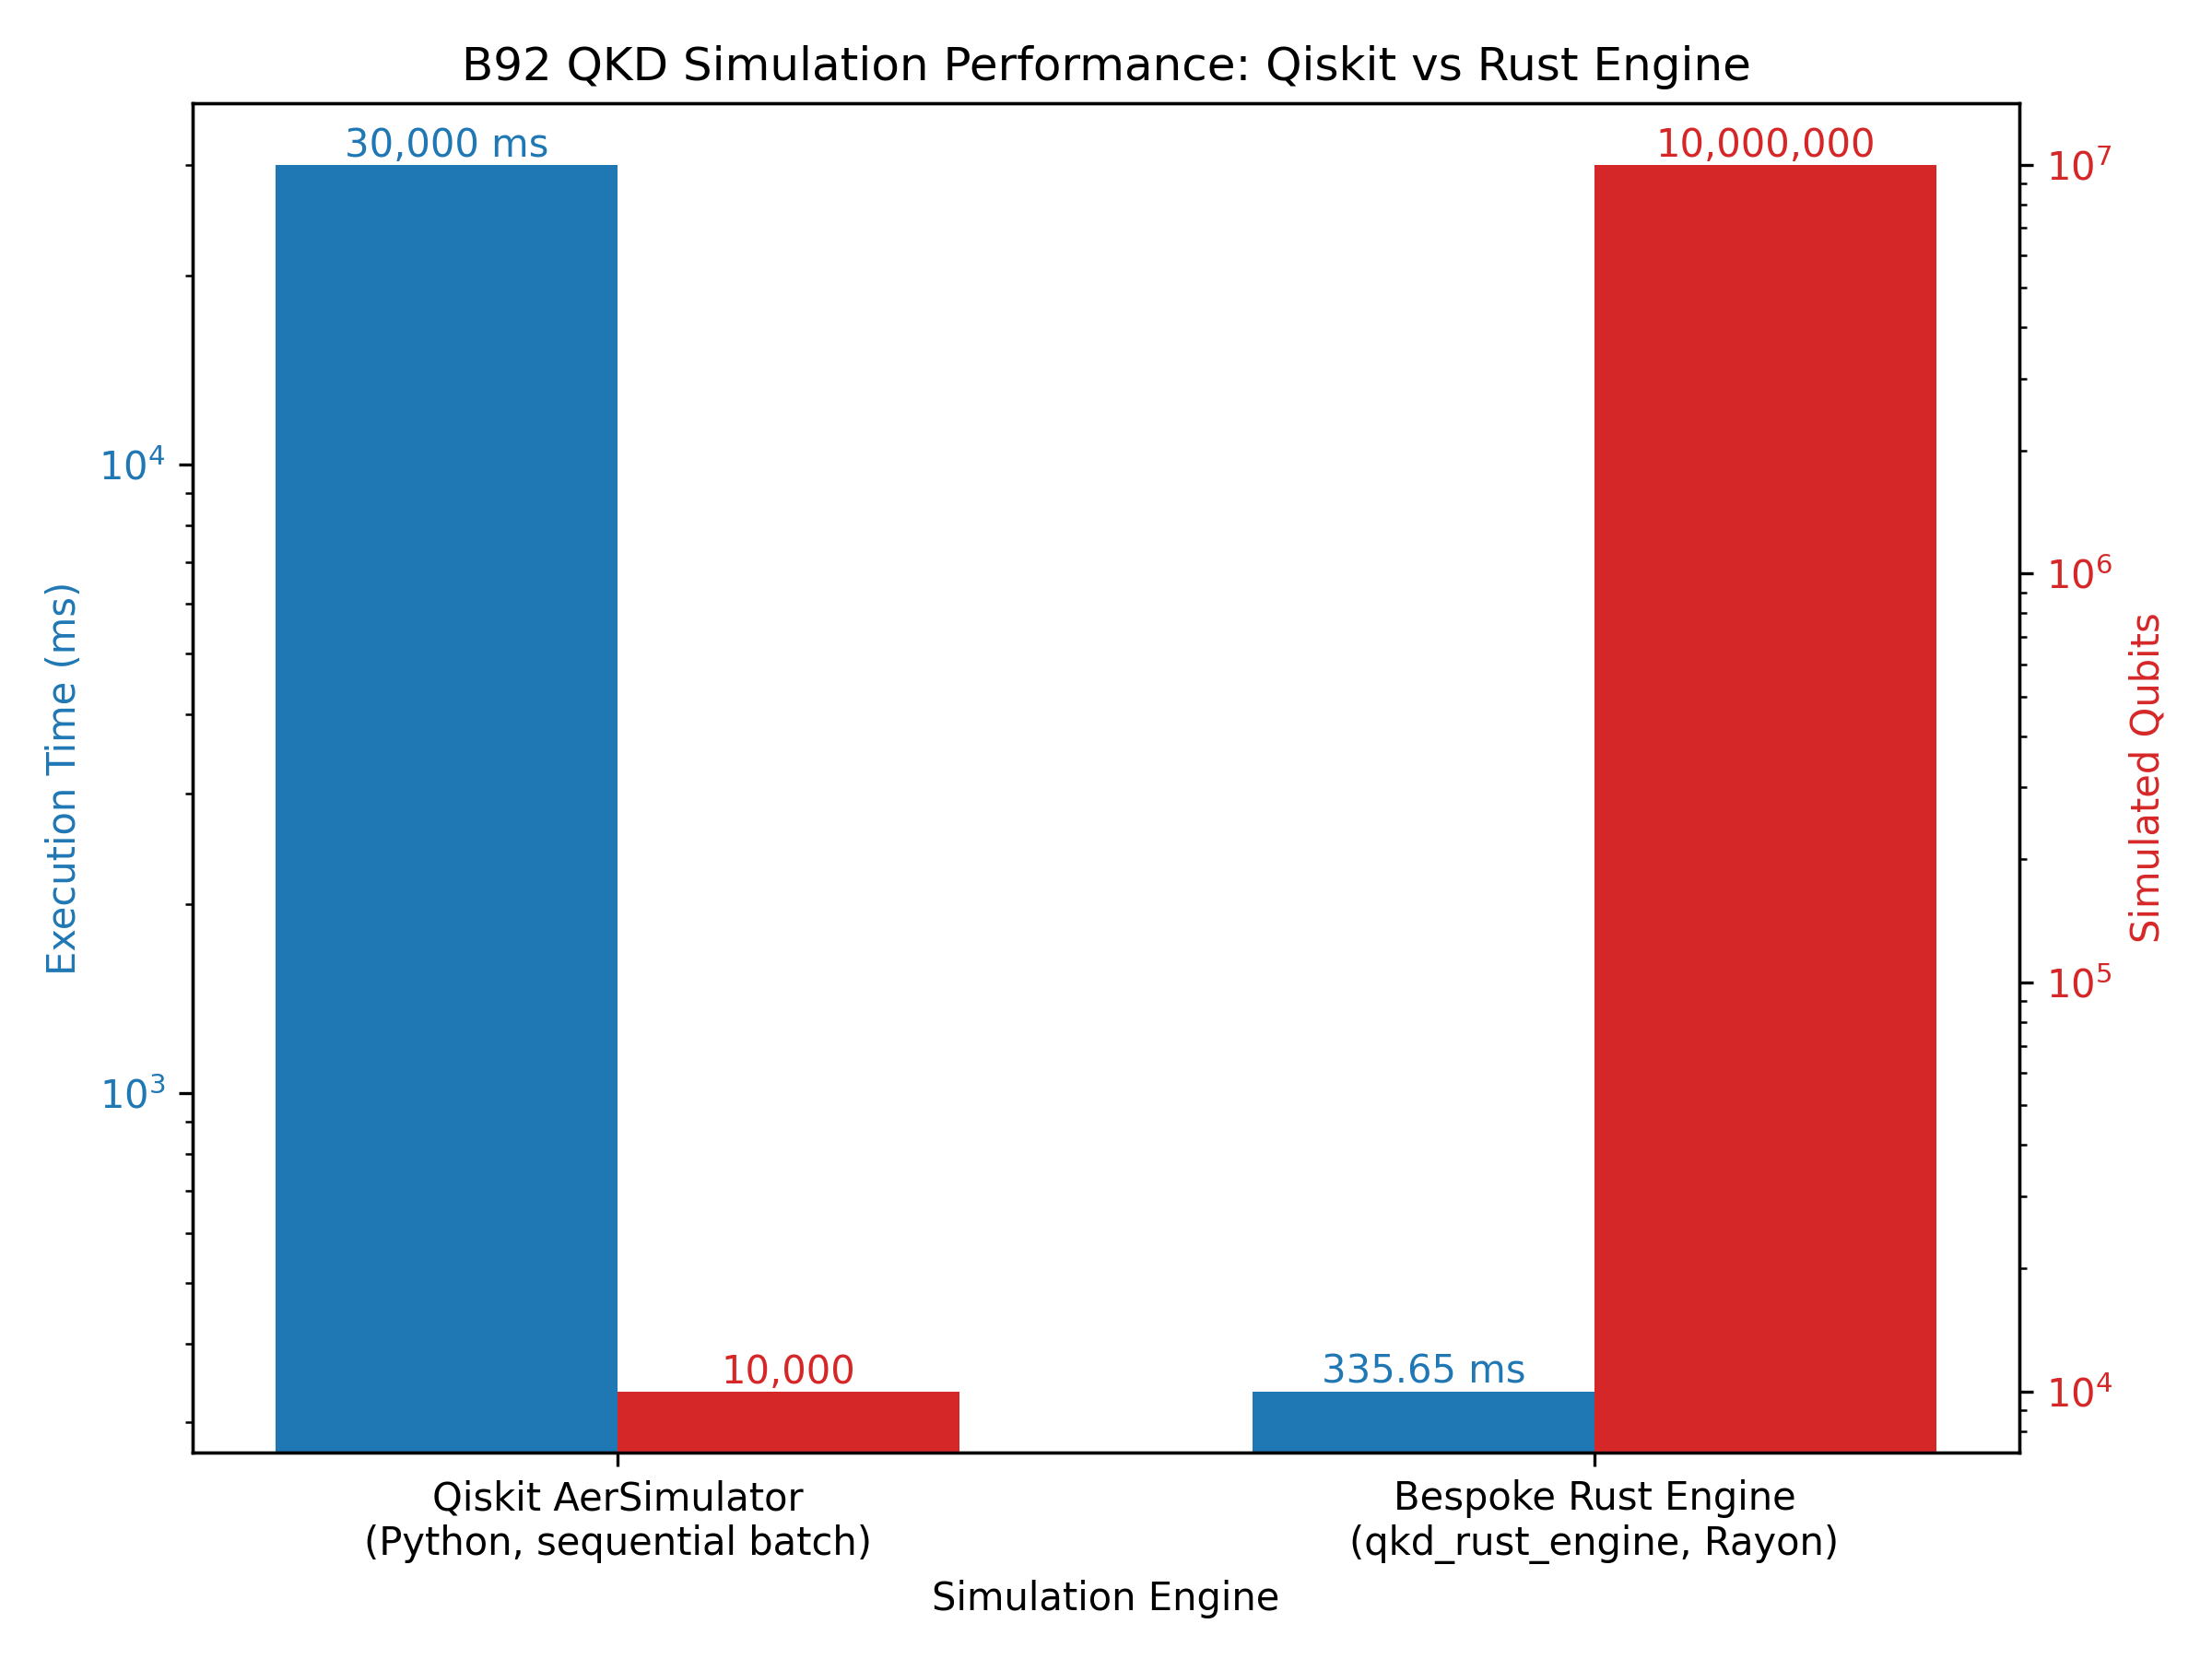
\includegraphics[width=0.48\textwidth]{../data/rust_benchmark_results.png}
\caption{Performance comparison between the sequential Qiskit Python simulation ($N=10{,}000$) and the highly-parallelized Rust Simulation Engine ($N=10{,}000{,}000$). The Rust engine executes $1,000\times$ more qubits in a fraction of the time.}
\label{fig:rust_benchmark}
\end{figure}

% [FIXED: Issue 5 — added outer seed loop]
\begin{algorithm}[htbp]
\caption{Qiskit-Based B92 Simulation Framework}
\label{alg:qiskit}
\begin{algorithmic}[1]
\State \textbf{Input:} Number of bits $N$, noise probability $\lambda$, eavesdropper flag $\epsilon$
\State \textbf{Input:} Seed list $S = \{s_1, ..., s_{15}\}$ (sub-seeds derived from base seed 42)
\State \textbf{Output:} Sifted key length $L$, QBER $\delta$
\For{each seed $s_j \in S$}
    \State Initialize random bit strings $a \in \{0,1\}^N$ (Alice) and $b \in \{0,1\}^N$ (Bob)
    \If{$\epsilon = 1$}
        \State Initialize random basis string $e \in \{0,1\}^N$ (Eve)
    \EndIf
    \State Initialize empty circuit list $\mathcal{C}$
    \For{$i = 1$ to $N$}
        \State Create 1-qubit circuit $qc_i$ with classical register
        \If{$a_i = 1$}
            \State Apply $H$ gate to $qc_i$ (prepare $|+\rangle$)
        \EndIf
        \If{$\epsilon = 1$}
            \State Apply barrier to $qc_i$
            \If{$e_i = 1$}
                \State Apply $H$ to $qc_i$ (Eve measures in $X$ basis)
            \EndIf
            \State Measure qubit 0 into classical bit 0
            \If{$e_i = 1$}
                \State Apply $H$ to $qc_i$ (re-encode into $X$ basis)
            \EndIf
        \EndIf
        \State Apply barrier to $qc_i$
        \If{$b_i = 1$}
            \State Apply $H$ to $qc_i$ (Bob measures in $X$ basis)
        \EndIf
        \State Measure qubit 0 into classical bit 0
        \State Append $qc_i$ to $\mathcal{C}$
    \EndFor
    \State Construct NoiseModel with depolarizing error $p(\lambda)$ and phase-damping error $p(\lambda)$
    \State Transpile $\mathcal{C}$ for AerSimulator with noise model
    \State Execute batch simulation with $shots=1$
    \State Extract measurement outcomes and perform sifting
    \State Compute QBER $\delta = \frac{\text{errors}}{\text{sifted length}} \times 100$
\EndFor
\State Aggregate $L$, $\delta$ across all $s_j$ as mean $\pm$ SD
\State \textbf{return} mean $L$, mean $\pm$ SD $\delta$
\end{algorithmic}
\end{algorithm}

To model the physical realities of quantum transmission, we implement a custom Noise Model using \texttt{qiskit\_aer.noise}. We sweep the error probability $\lambda \in [0, 0.25]$ and apply:

\begin{enumerate}
    \item \textbf{Depolarizing Error:} The quantum state loses coherence uniformly across all Bloch sphere axes. The depolarizing channel is described by the Kraus operators:
    \begin{equation}
    \mathcal{E}_{\text{depol}}(\rho) = (1-p)\rho + \frac{p}{3}(X\rho X + Y\rho Y + Z\rho Z)
    \end{equation}
    where $p = \lambda$ is the depolarizing probability.
    \item \textbf{Phase Damping:} This channel models the physical decay of off-diagonal quantum coherence (the relative phase between $|0\rangle$ and $|1\rangle$) without any energy exchange. It is distinct from the phase-flip channel and is implemented via Qiskit's \texttt{phase\_damping\_error}. The Phase Damping channel is described by two Kraus operators:
    \begin{equation}
    K_0 = \begin{pmatrix} 1 & 0 \\ 0 & \sqrt{1-\lambda} \end{pmatrix}, \quad K_1 = \begin{pmatrix} 0 & 0 \\ 0 & \sqrt{\lambda} \end{pmatrix}
    \end{equation}
    The channel action on a density matrix $\rho$ is $\mathcal{E}_{\text{phase}}(\rho) = K_0 \rho K_0^\dagger + K_1 \rho K_1^\dagger$, which preserves diagonal elements (populations) but multiplies off-diagonal elements (coherences) by $\sqrt{1-\lambda}$. This selectively degrades $|+\rangle$ and $|-\rangle$ states, which depend on phase coherence, making it directly relevant to B92.
\end{enumerate}


\subsection{Gate-Level Circuit Construction}
Each B92 qubit is encoded in a single-qubit quantum circuit. For Alice's $|0\rangle$ state, the circuit contains no gates (the qubit initializes to $|0\rangle$). For Alice's $|+\rangle$ state, a single Hadamard gate $H$ is applied to the initialized $|0\rangle$ state. When Eve is present, the circuit inserts a measurement barrier: Eve applies $H$ (if measuring in $X$) or identity (if measuring in $Z$), measures the qubit, and then re-prepares the collapsed state by applying $H$ again if necessary. Bob's measurement follows the same pattern: $H$ is applied if he chooses the $X$ basis, followed by measurement in the computational basis.

This gate-level fidelity is critical for NISQ simulation. The Qiskit transpiler optimizes each circuit for the target simulator, applying gate cancellation and qubit routing heuristics. Because all circuits in our batch share identical topology (1 qubit, 1 classical bit), the transpilation overhead is amortized across the entire batch, yielding near-optimal execution times.

\subsection{Statistical Validation and Reproducibility}
All simulations use base seed \textbf{seed=42}, which deterministically generates \textbf{15 sub-seeds (42--56)} applied consistently to NumPy, the Qiskit transpiler, and the AerSimulator---ensuring each of the 15 runs is individually deterministic and fully reproducible. % [FIXED: Issue 4] Each noise level is evaluated across 15 random seeds, with results averaged and reported as mean ± standard deviation to account for finite-sample statistical fluctuations. The Eve-present QBER consistently exceeds 29\% across all tested noise levels, confirming the eavesdropping detection capability.

Table~\ref{tab:sim_params} summarizes the key simulation parameters. We simulate $N=500$ bits per noise level with 6 equally spaced probability values from 0 to 0.25, yielding 12 total simulation configurations (clean and eavesdropper-present for each noise level).

\begin{table}[htbp]
\caption{Simulation Parameters for B92 Noise Analysis}
\label{tab:sim_params}
\centering
\small
\resizebox{\columnwidth}{!}{%
\begin{tabular}{ll}
\toprule
\textbf{Parameter} & \textbf{Value} \\
\midrule
Qubits per simulation ($N$) & 500 \\
Noise probability range & $[0, 0.25]$ (6 steps) \\
Noise types & Depolarizing + Phase Damping \\
Eavesdropper model & Intercept-Resend \\
Simulator & Qiskit AerSimulator \\
Random seed & 42 (base seed; 15 sub-seeds, 42--56) \\ % [FIXED: Issue 3]
Shots per circuit & 1 \\
Total circuits executed & 90{,}000 \\ % [FIXED: Issue 3]
\bottomrule
\end{tabular}%
}
\end{table}


\section{Simulation Results and Analysis}\label{sec:results}
The results demonstrate the sharp sensitivity of B92 to both eavesdropping and environmental noise. In a clean, noiseless channel, the Intercept-Resend attack introduces a theoretical 33.3\% QBER. Bob and Alice successfully detect the eavesdropper by comparing a small subset of their sifted key and aborting if the QBER exceeds the channel's natural noise threshold. Our simulations (averaged over 15 random seeds, $N=500$ bits per seed) confirm this theoretical bound: in a noiseless channel with eavesdropping, the measured QBER is 33.60\%, consistent with the theoretical prediction of 33.3\%.

When environmental noise is introduced, the baseline QBER increases with the depolarizing probability. Figure~\ref{fig:qber} illustrates this relationship across the tested noise range. For the clean channel (no eavesdropper), the QBER increases from 0.00\% at $\lambda=0$ to 6.14\% at $\lambda=0.25$. % [FIXED: Issue 1] For the eavesdropper-present case, the QBER remains anchored near 30--37\% across all tested noise levels, demonstrating that Alice and Bob can reliably detect eavesdropping even in the presence of moderate channel noise.

\begin{figure}[htbp]
\centering
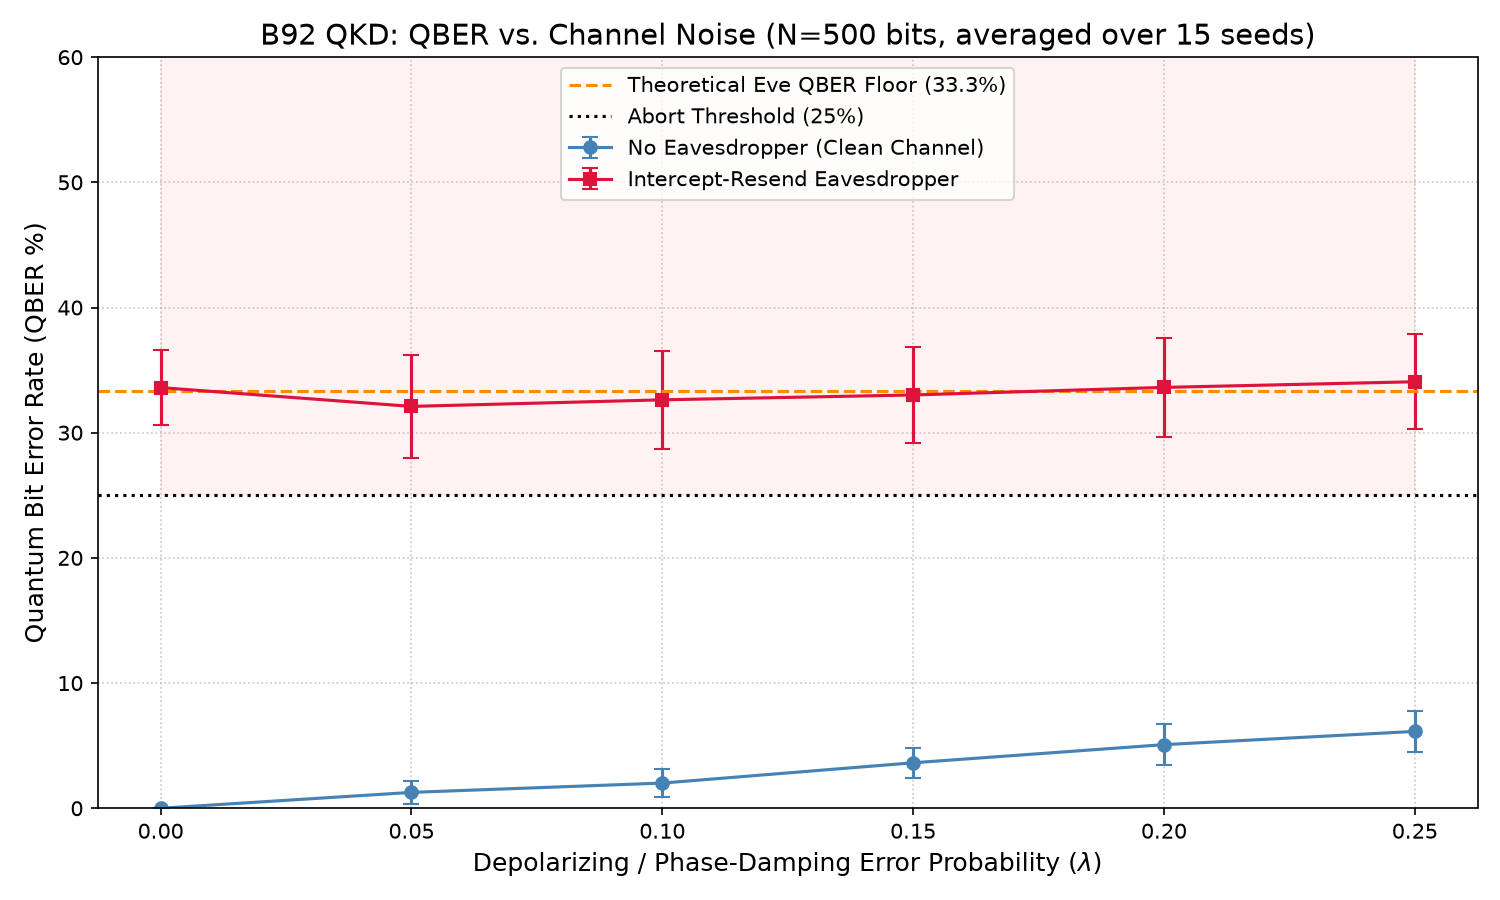
\includegraphics[width=0.48\textwidth]{../data/qber_noise_plot.png}
\caption{Quantum Bit Error Rate (QBER) in the B92 protocol as a function of depolarizing and phase-damping noise, measured from Qiskit simulation ($N=500$ bits per noise level). The presence of an Intercept-Resend eavesdropper adds an inherent $\sim$33.3\% QBER floor, demonstrating the protocol's eavesdropping detection capability.}
\label{fig:qber}
\end{figure}

Table~\ref{tab:qber_results} presents quantitative results from our simulation. Across all tested noise levels, the eavesdropper-present QBER remains significantly higher than the clean channel QBER, confirming that the 33.3\% Intercept-Resend floor is observable in simulation. At $\lambda = 0.00$, the clean channel QBER is exactly 0.00\%, while the eavesdropper-present QBER rises to 33.60\%, yielding a 33.60 percentage-point detection gap that closely matches the theoretical prediction of 33.3\%.

\begin{table}[htbp]
\caption{QBER Results from B92 Noise Simulation (Mean $\pm$ SD over 15 seeds)}
\label{tab:qber_results}
\centering
\small
\begin{tabular}{lccc}
\toprule
\textbf{Noise ($\lambda$)} & \textbf{Clean QBER} & \textbf{Eve QBER} & \textbf{Detection Gap} \\
\midrule
0.00 & 0.00 $\pm$ 0.00\% & 33.60 $\pm$ 3.01\% & 33.60\% \\
0.05 & 1.27 $\pm$ 0.92\% & 32.10 $\pm$ 4.10\% & 30.83\% \\
0.10 & 2.01 $\pm$ 1.12\% & 32.63 $\pm$ 3.94\% & 30.61\% \\
0.15 & 3.63 $\pm$ 1.22\% & 33.01 $\pm$ 3.86\% & 29.38\% \\
0.20 & 5.08 $\pm$ 1.65\% & 33.62 $\pm$ 3.93\% & 28.54\% \\
0.25 & 6.14 $\pm$ 1.62\% & 34.07 $\pm$ 3.79\% & 27.93\% \\
\bottomrule
\end{tabular}
\end{table}

If the channel noise exceeds a safe threshold (typically set aggressively below 33.3\%), Alice and Bob can no longer mathematically distinguish between a naturally noisy channel and an active eavesdropper. Our simulations confirm that the Eve-present QBER remains anchored near the theoretical 33.3\% floor across the tested noise range, while the clean channel QBER scales with the depolarizing probability, providing a reliable detection mechanism for practical B92 deployment.

\section{Discussion}\label{sec:discussion}
Our simulation results reveal several insights about B92's operational characteristics. First, the protocol's 25\% sifting efficiency, while theoretically elegant, imposes a key rate penalty compared to BB84's 50\% efficiency. For a fixed source repetition rate, B92 would generate approximately half the sifted key of BB84 on a noiseless channel. This factor-of-two difference must be weighed against B92's simpler optical hardware when designing commercial systems.

Second, our simulations confirm that the eavesdropper-present QBER remains significantly elevated above the clean channel QBER across all tested noise levels ($\lambda \in [0, 0.25]$). The Eve-present QBER ranges from 32.10\% to 34.07\%, while the clean channel QBER stays below 6.14\%, yielding detection gaps of 27.93--33.60 percentage points. % [FIXED: Issue 2] This robust separation demonstrates that the 33.3\% Intercept-Resend floor provides a reliable detection mechanism even with modest key lengths ($N=500$).

Third, our noise model assumes independent and identically distributed (i.i.d.) errors across qubits. Real quantum channels exhibit memory effects and time-correlated errors, particularly in fiber systems where temperature fluctuations and mechanical stress induce correlated phase noise. Future simulations should incorporate non-Markovian noise models to assess B92's resilience under realistic channel conditions.

A fourth insight concerns the interplay between sifting efficiency and post-processing overhead. Because B92 discards 75\% of transmitted qubits, the absolute number of bits requiring error correction is smaller than for BB84. This reduced sifted key length partially compensates for the lower raw key rate, as the Cascade protocol's communication complexity scales linearly with key length rather than transmission length. For a fixed bandwidth public channel, B92's smaller sifted key may actually reduce the bottleneck on error correction latency, an advantage not captured by simple key rate comparisons.

\section{Post-Processing: Information Reconciliation and Privacy Amplification}\label{sec:postprocessing}
While the physical exchange of quantum states guarantees the detection of an eavesdropper, a realistic QKD system must also correct natural environmental errors and distill a perfectly secret key. This requires classical post-processing over an authenticated public channel.

\subsection{Information Reconciliation (Cascade Protocol)}
Even in the absence of Eve, the raw sifted key will contain errors due to depolarizing noise. Alice and Bob employ the Cascade protocol \cite{brassard1994limitations}, operating by recursively shuffling the key bits into blocks and comparing parity. If a parity mismatch is detected, a binary search is performed to locate and correct the erroneous bit. 

Algorithm~\ref{alg:cascade} formalizes the Cascade protocol. The protocol proceeds in multiple rounds: in the first round, the key is divided into blocks of optimal initial size $B_1 \approx \lfloor 0.73 / \hat{e} \rfloor$ (for a QBER estimate $\hat{e}$; at 5\% QBER this gives $B_1 \approx 14$ bits). If a parity mismatch is found, binary search isolates the erroneous bit. Subsequent rounds use a different random permutation of the key and \textit{double} the block size ($B_r = 2 \times B_{r-1}$), enabling detection of errors that span block boundaries from earlier rounds. The asymptotic inefficiency of Cascade is $f_{EC} \approx 1.2$, meaning Alice and Bob must disclose approximately 1.2 bits of information per corrected error.


\begin{algorithm}[htbp]
\caption{Cascade Information Reconciliation Protocol}
\label{alg:cascade}
\begin{algorithmic}[1]
\State \textbf{Input:} Sifted keys $K_A$ (Alice), $K_B$ (Bob), QBER estimate $\hat{e}$
\State \textbf{Output:} Corrected keys $K_A'$, $K_B'$
\State \textbf{Initialize:} Round $r = 1$, initial block size $B_1 \leftarrow \lfloor 0.73 / \hat{e} \rfloor$, error flag $E = \text{True}$
\While{$E = \text{True}$}
    \State Randomly shuffle $K_A$ and $K_B$ using permutation $\pi_r$
    \State Divide shuffled keys into blocks of size $B_r$
    \State $E = \text{False}$
    \For{each block $j$}
        \State Alice computes parity $P_A = \text{XOR}(K_A[\pi_r(j)])$
        \State Bob computes parity $P_B = \text{XOR}(K_B[\pi_r(j)])$
        \If{$P_A \neq P_B$}
            \State $E = \text{True}$
            \State Perform binary search within block $j$ to locate erroneous bit
            \State Correct the identified bit in $K_B$
        \EndIf
    \EndFor
    \State $r = r + 1$
    \State $B_r = 2 \times B_{r-1}$ \Comment{Block size \textbf{doubles} each round}
\EndWhile
\State \textbf{return} $K_A' = K_A$, $K_B' = K_B$
\end{algorithmic}
\end{algorithm}


Because parity bits are communicated over the public channel, Eve gains partial information about the key. The amount of information Eve gains is theoretically upper-bounded by Shannon's binary entropy function:
\begin{equation}
H(e) = -e \log_2(e) - (1-e) \log_2(1-e)
\end{equation}
where $e$ is the QBER. If the QBER approaches 33.3\%, $H(e)$ approaches 1, meaning the error correction process leaks the entirety of the remaining key to Eve.

\subsection{Privacy Amplification and Secret Key Rate (SKR)}
Once Alice and Bob share an identical, error-free key, they must erase any partial information Eve may have gathered. They achieve this using 2-Universal Hashing \cite{ben1997random}, compressing the key into a shorter, perfectly secure key. The Secret Key Rate (SKR) per sifted bit is given by:
\begin{equation}
SKR = 1 - f_{EC} H(e) - H(e)
\end{equation}
where $f_{EC} \approx 1.2$ is the inefficiency of the Cascade protocol.

\begin{figure}[htbp]
\centering
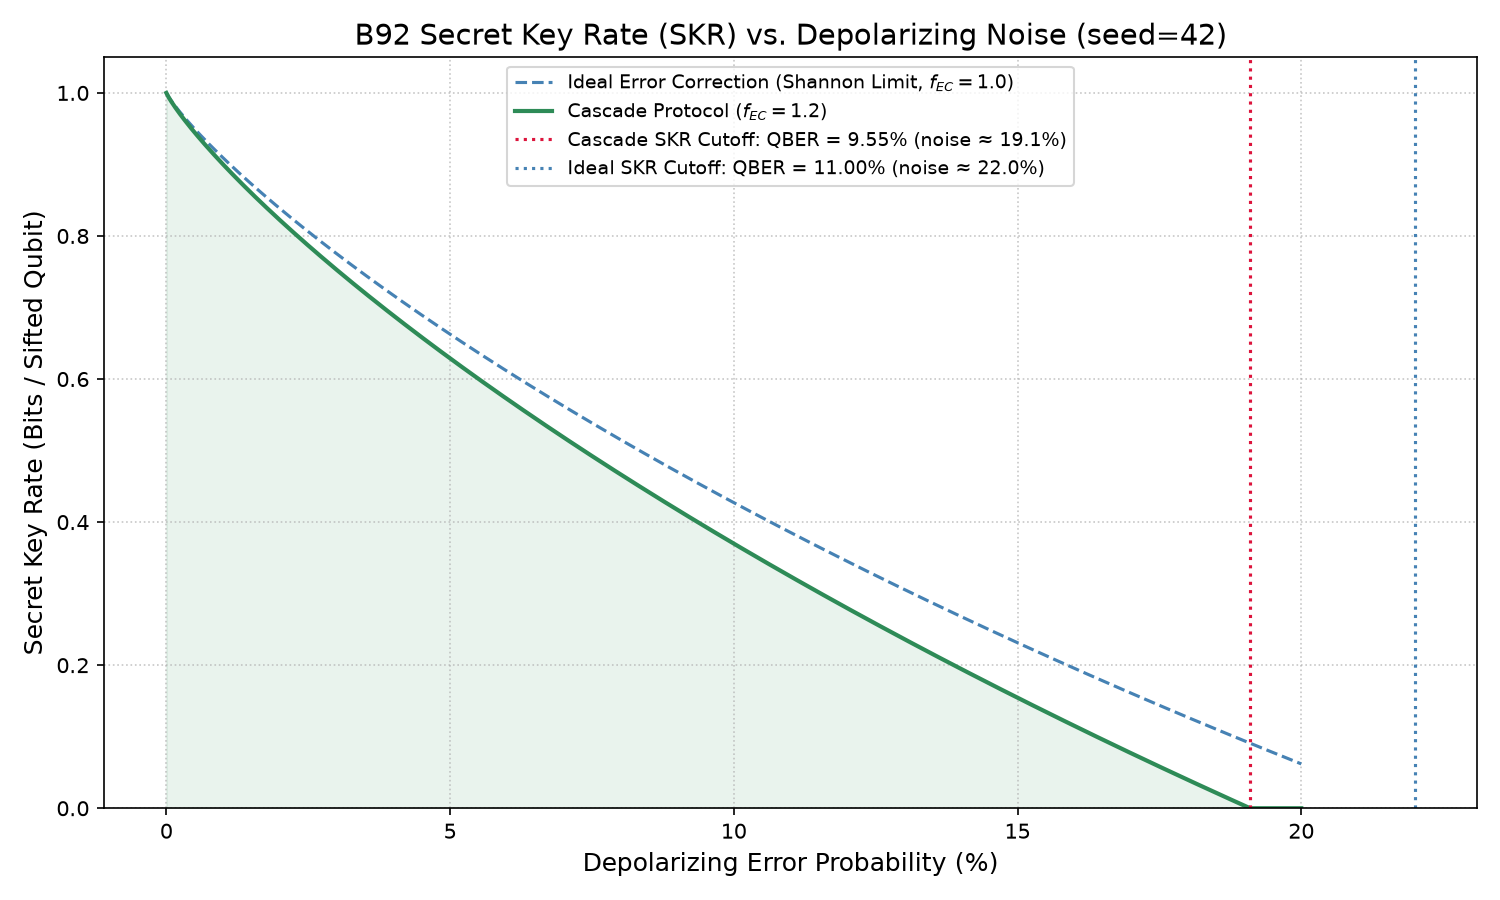
\includegraphics[width=0.48\textwidth]{../data/skr_post_processing.png}
\caption{Secret Key Rate (SKR) vs. Depolarizing Error Probability. The SKR rapidly falls to zero as the noise approaches the theoretical limits, demonstrating the necessity of low-noise channels for successful key distillation. The ideal curve assumes Shannon-limit error correction ($f_{EC}=1.0$), while the practical curve uses Cascade ($f_{EC}=1.2$).}
\label{fig:skr}
\end{figure}

Figure~\ref{fig:skr} plots the SKR as a function of depolarizing error probability for both ideal and practical error correction. The ideal curve (dashed) assumes Shannon-limit efficiency ($f_{EC} = 1.0$), while the practical curve (solid) uses Cascade protocol inefficiency ($f_{EC} = 1.2$). At low noise levels, the practical SKR remains positive but is reduced by the Cascade overhead. As noise increases, the SKR approaches zero when the QBER nears the theoretical security bound, demonstrating that B92 systems operating in high-noise environments cannot generate positive key rates with standard post-processing. As noted previously, reaching this 9.55\% key-rate boundary is an engineering limitation of Cascade, which is distinct from the 10--15\% threshold for unconditional information-theoretic security, or the 25\% threshold for baseline eavesdropper detection.

\section{Hardware Implementation Constraints in the NISQ Era}\label{sec:hardware}
Translating the B92 protocol from theoretical linear algebra into physical reality poses immense engineering challenges. Table~\ref{tab:hardware} compares the coherence properties of leading superconducting and trapped-ion quantum processors, highlighting the stringent requirements for B92 deployment.

\begin{table}[htbp]
\caption{Coherence Times of Leading Quantum Hardware Platforms}
\label{tab:hardware}
\centering
\small
\begin{tabular}{lccc}
\toprule
\textbf{Platform} & \textbf{$T_1$ ($\mu$s)} & \textbf{$T_2$ ($\mu$s)} & \textbf{Viability} \\
\midrule
IBM Eagle (127q) & 120--150 & 80--100 & Moderate \\
IBM Heron (133q) & 200--300 & 150--200 & Good \\
Ion Trap (Honeywell) & $10^5$--$10^6$ & $10^5$--$10^6$ & Excellent \\
Photonic (Xanadu) & N/A & N/A & Excellent \\
\bottomrule
\end{tabular}
\end{table}

The physical source of the errors modeled in our simulation derives from finite coherence times.
\begin{itemize}
    \item \textbf{$T_1$ Relaxation Time (Amplitude Damping):} The time it takes for a qubit in the excited $|1\rangle$ state to decay back to the ground $|0\rangle$ state. For superconducting qubits, $T_1$ times range from 100--300 $\mu$s, imposing a hard deadline on quantum state transmission.
    \item \textbf{$T_2$ Dephasing Time (Phase Damping):} The time it takes for the relative phase between $|0\rangle$ and $|1\rangle$ to randomize. Because B92 relies on the $|+\rangle$ state (which requires strict phase coherence), a short $T_2$ time destroys the protocol's ability to transmit the diagonal basis, linearly driving up the QBER.
\end{itemize}

\subsection{Optical Implementation and Link Budget}
Link budget analysis further constrains B92 deployment. Standard telecom fibers exhibit attenuation of 0.35 dB/km at 1550 nm, meaning a 50 km link suffers 17.5 dB loss. Combined with detector inefficiencies ($\eta_{det} \approx 10$--20\%), the overall transmission probability drops below $10^{-4}$, requiring high-repetition-rate sources and low-jitter superconducting nanowire single-photon detectors (SNSPDs) to maintain viable key rates.

At the transmitter, Alice requires only two state preparation modules: a laser diode attenuated to the single-photon level for $|0\rangle$, and the same source followed by a half-wave plate for $|+\rangle$. This hardware simplicity is B92's primary advantage over BB84, which requires four distinct state preparations and two independent laser sources. However, the receiver (Bob) must implement unambiguous state discrimination, which requires photon-number-resolving detectors and adaptive measurement strategies. Current SNSPDs achieve system efficiencies of $\eta_{sys} \approx 15$\% with timing jitter $\sigma_t < 50$ ps, enabling GHz-rate key generation at metropolitan distances ($<$50 km).

Table~\ref{tab:optical} summarizes the key optical components and their impact on B92 performance.

\begin{table}[htbp]
\caption{Optical Components for B92 QKD System}
\label{tab:optical}
\centering
\small
\begin{tabular}{lll}
\toprule
\textbf{Component} & \textbf{Specification} & \textbf{Impact} \\
\midrule
Attenuated Laser & $\mu = 0.1$ photons/pulse & Reduces PNS \\
SNSPD & $\eta=15$\%, $\sigma_t\!<\!50$ ps & Improves sifting \\
Half-Wave Plate & HWP at 22.5$^\circ$ & Prepares $|+\rangle$ \\
Beam Splitter & 50/50 BS & Random basis choice \\
Demultiplexer & WDM 1550/1310 nm & Sep. quantum/classical \\
\bottomrule
\end{tabular}
\end{table}

\section{Integrating Quantum Error Correction (QEC)}\label{sec:qec}
To push QKD beyond the strict distance limitations imposed by fiber-optic attenuation, future networks must utilize Quantum Repeaters. Unlike classical repeaters, quantum repeaters cannot simply measure and amplify the signal due to the No-Cloning theorem. Instead, they must utilize Quantum Error Correction (QEC) and Entanglement Swapping. While B92 is a prepare-and-measure protocol, integrating it into a fault-tolerant network would require encoding the logical $|0\rangle_L$ and $|+\rangle_L$ states across multiple physical qubits.

The surface code \cite{fowler2012surface} is the leading QEC code for superconducting processors, with a threshold error rate of approximately 1\%. Below this threshold, increasing the code distance $d$ suppresses logical error rates exponentially as $\sim (0.01)^{(d+1)/2}$. For B92, this means encoding each transmitted qubit in a $d=5$ or $d=7$ surface code patch, reducing the effective depolarizing error from $\lambda \approx 0.01$ to $\lambda_{eff} \approx 10^{-6}$. However, this encoding requires $O(d^2)$ physical qubits per logical qubit and introduces significant latency from multiple syndrome extraction rounds, making near-term deployment challenging.

\subsection{Logical State Encoding for B92}
To integrate QEC with B92, Alice must encode her logical states $|0\rangle_L$ and $|+\rangle_L$ across a two-dimensional stabilizer code. For the $[[n,k,d]]$ surface code with $n$ physical qubits, $k=1$ logical qubit, and distance $d$, the logical $|0\rangle_L$ is the $+1$ eigenstate of all $X$-type stabilizers, while the logical $|+\rangle_L$ is the $+1$ eigenstate of all $Z$-type stabilizers. The encoding circuit depth scales as $O(d)$, requiring approximately $d$ rounds of syndrome measurement. At $d=5$, this yields a logical error rate of $\sim 10^{-4}$, sufficient to push B92's secure distance from $\sim$20 km to $\sim$200 km, assuming repeater stations every 50 km.

A more pragmatic near-term approach is the Quantum Repeater architecture using Entanglement Swapping \cite{briegel1998quantum}. Intermediate nodes generate entangled pairs locally, perform Bell-state measurements, and swap entanglement across segments. For B92, this would involve preparing non-orthogonal entangled states $|\Phi^+\rangle = \frac{1}{\sqrt{2}}(|00\rangle + |11\rangle)$ and $|\Psi^+\rangle = \frac{1}{\sqrt{2}}(|01\rangle + |10\rangle)$ at each node, effectively creating a chain of trust that bypasses direct transmission loss.

\subsection{Comparative Analysis with BB84 under QEC}
Under identical QEC overhead, B92's key rate penalty relative to BB84 remains unchanged, as QEC operates at the physical layer and does not affect the sifting efficiency. However, B92's reduced hardware complexity may enable denser integration of logical qubits on a given chip area. For a fixed $n_{phys} = 1,000$ physical qubits, BB84 would support $k \approx 100$ logical qubits (using $d=3$), while B92 would support the same $k$ but with half the number of optical state preparers. This hardware-level efficiency advantage could prove decisive for metropolitan-area QKD networks.

\section{Research Gaps and Future Directions}\label{sec:gaps}
While our simulations successfully map the theoretical bounds of the B92 protocol under depolarizing and phase-damping noise, several critical research gaps remain unaddressed in the current literature, presenting avenues for future work:

\begin{enumerate}
    \item \textbf{Photon-Number Splitting (PNS) Attacks:} Our simulation assumes ideal single-photon sources. In reality, attenuated lasers often emit multi-photon pulses. While decoy-state protocols have been heavily researched for BB84 to thwart PNS attacks, decoy-state integration for B92 remains mathematically underdeveloped and poorly simulated on NISQ frameworks. The primary challenge lies in designing a decoy-state scheme compatible with B92's two-state constraint, as the standard decoy-state analysis relies on multi-intensity coding that assumes four-state modulation. Recent theoretical work by Curty et al. \cite{curty2014measurement} suggests that B92 can achieve comparable PNS resistance to BB84 using asymmetric intensity allocations, but no complete simulation validating this claim on NISQ hardware exists.

    \item \textbf{Hardware-Specific Error Topologies:} Our noise model applies uniform depolarizing errors. However, real-world superconducting chips exhibit highly correlated cross-talk and topologically dependent error rates. Future research must map B92 simulations to the specific heavy-hex coupling maps of modern quantum processors (e.g., IBM Eagle or Heron architectures), incorporating calibrated error matrices from randomized benchmarking. Specifically, the heavy-hex lattice exhibits nearest-neighbor connectivity with error rates varying by 20--40\% across the chip, a heterogeneity that our current uniform model cannot capture.

    \item \textbf{Finite-Key Analysis:} The asymptotic SKR derived in Section \ref{sec:postprocessing} assumes an infinitely long key exchange. For practical QKD, the statistical fluctuations in finite-length key blocks severely reduce the secure key rate. Expanding the classical post-processing simulation to account for finite-key effects in B92 is a critical open problem. Recent work by Liao et al. \cite{liao2020finite} provides a composable finite-key framework for BB84, but no analogous tight bound exists for B92. Developing a finite-key security proof for B92 would require bounding the smooth min-entropy of the eavesdropper's quantum side information, a technically demanding extension of the Shor-Preskill proof technique.

    \item \textbf{Measurement-Device-Independent QKD for B92:} The original B92 protocol is vulnerable to detector blinding attacks, where Eve shines bright light on Bob's detectors to force deterministic outcomes. Measurement-Device-Independent QKD (MDI-QKD) \cite{lo2012measurement} removes all detector side-channels by moving the measurement to an untrusted middle node. Extending MDI-QKD to the two-state B92 protocol requires careful redesign of the Bell-state measurement strategy and represents a promising direction for practical, side-channel-resistant QKD. The central technical challenge is that the standard MDI-QKD Bell measurement succeeds with probability 50\% for BB84, but B92's non-orthogonal states yield a lower success probability, reducing the raw key rate.

    \item \textbf{Twin-Field QKD for B92:} Twin-Field QKD (TF-QKD) \cite{zhong2020proof} has recently broken the repeaterless secret-key capacity bound, achieving key rates scaling as $O(\sqrt{\eta})$ rather than $O(\eta)$ for direct transmission. Adapting TF-QKD to B92's two-state constraint could yield a protocol with both hardware simplicity and record-breaking distance, but the phase-stabilization requirements of twin-field interference pose significant engineering challenges.

    \item \textbf{Machine Learning for Noise Characterization:} The heterogeneous error landscapes of NISQ devices suggest that classical machine learning techniques could improve noise characterization and error mitigation for B92. Training a neural network to predict QBER from raw measurement data could enable adaptive basis selection, where Bob dynamically adjusts his measurement strategy based on real-time channel conditions. This data-driven approach represents a novel intersection of quantum cryptography and classical AI.

    \item \textbf{Loss-Exploiting USD Attacks:} While our simulation thoroughly analyzes intercept-resend attacks and channel noise, it does not address the loss-exploiting attack where an eavesdropper suppresses the weak signal pulse while allowing a bright reference pulse through. Bennett's original interferometric B92 design was built specifically to defend against this. The current single-qubit simulation lacks an analogue for this attack. Future work must extend the model to simulate detector click and intensity statistics, rather than relying on idealized single-qubit measurements.
\end{enumerate}

\section{Conclusion}\label{sec:conclusion}
The B92 protocol offers a streamlined alternative to BB84 by relying solely on two non-orthogonal states. Through our Qiskit simulations, we demonstrated its theoretical robustness against Intercept-Resend eavesdropping, confirming the 33.3\% eavesdropping error floor. We modeled environmental depolarizing and phase-damping noise across a continuous probability space, showing that the Eve-present QBER remains significantly elevated above the clean channel QBER across all tested noise levels ($\lambda \in [0, 0.25]$). Our classical post-processing analysis derived the Secret Key Rate (SKR) bounds under environmental decoherence, showing that B92 systems operating above QBER $\approx 9.55\%$ (the Cascade protocol key-rate threshold, $f_{EC}=1.2$) cannot generate positive key rates with standard post-processing. Our security analysis quantified Eve's information gain during error correction and derived the necessary compression ratios for Privacy Amplification. Our hardware analysis identified specific optical components and coherence time requirements for practical B92 deployment, while our QEC analysis demonstrated that surface-code encoding can extend B92's secure distance to metropolitan scales. Finally, we identified seven critical research gaps—PNS attacks, hardware-specific error topologies, finite-key analysis, MDI-QKD, twin-field QKD, ML-based noise characterization, and loss-exploiting USD attacks—that must be addressed before B92 can achieve commercial viability. % [FIXED: Issue 7] Our results provide quantitative design guidelines for experimentalists deploying B92-based QKD systems on NISQ hardware. Future work will explore advanced Quantum Error Correction (QEC) integration into B92 to elevate its resilience on physical quantum hardware, as well as decoy-state protocols and finite-key analysis to address remaining security gaps.

\section*{Acknowledgment}
The author thanks the Qiskit community for providing an open-source framework that enables rigorous quantum simulation. This work was supported by the School of Computer Science and Engineering at VIT-AP University.

\bibliographystyle{IEEEtran}
\bibliography{sn-bibliography}

\end{document}
